% This is samplepaper.tex, a sample chapter demonstrating the
% LLNCS macro package for Springer Computer Science proceedings;
% Version 2.20 of 2017/10/04
%
\documentclass[runningheads]{llncs}
%

\makeatletter
\@ifclasswith{llncs}{peerreview}{
	\author{}
	\typeout{PEERREVIEW}
	\newcommand\MYhyperrefoptions{
		pdftitle={MessageVortex Protocol -- Sending Messages Anonymously},
		pdfsubject={MessageVortex Protocol},
		pdfkeywords={Messages, Unobservable, Anonymity, Unlinkability, Pseudonymity }
	}
}{
	\typeout{PUBLIC}
	\author{M. Gwerder\inst{1,2}\orcidID{0000-0003-0296-5079}}
	%
	\authorrunning{M. Gwerder}
	\institute{University of Basel, Switzerland \and
		University of Applied Sciences of Northwestern of Switzerland\\
		\email{martin.gwerder@fhnw.ch}\\
		%\url{https://www.fhnw.ch/en/about-fhnw/schools/school-of-engineering/institutes/institute-of-mobile-and-distributed-systems} 
	}
	\newcommand\MYhyperrefoptions{
		pdftitle={MessageVortex Protocol -- Sending Messages Anonymously},
		pdfsubject={MessageVortex Protocol},
		pdfkeywords={Messages, Unobservable, Anonymity, Unlinkability, Pseudonymity }
		pdfauthor={Martin Gwerder},%<!CHANGE
	}
}
\makeatother
\usepackage{xcolor}
\usepackage[\MYhyperrefoptions,pdftex]{hyperref}
\usepackage{graphicx}
\usepackage{appendix}

\usepackage[cmex10]{amsmath}
\DeclareMathOperator{\prng}{prng}
\DeclareMathOperator{\len}{len}
\DeclareMathOperator{\splitPayload}{splitPayload}
\DeclareMathOperator{\mergePayload}{mergePayload}
\DeclareMathOperator{\startsWith}{startsWith}
\DeclareMathOperator{\lendsWith}{endsWith}
\DeclareMathOperator{\addRedundancy}{addRedundancy}
\DeclareMathOperator{\removeRedundancy}{removeRedundancy}
\DeclareMathOperator{\encrypt}{encrypt}
\DeclareMathOperator{\decrypt}{decrypt}

\usepackage[pdftex]{thumbpdf}

\hyphenation{op-tical net-works semi-conduc-tor}

% Used for displaying a sample figure. If possible, figure files should
% be included in EPS format.
%
% If you use the hyperref package, please uncomment the following line
% to display URLs in blue roman font according to Springer's eBook style:
\renewcommand\UrlFont{\color{blue}\rmfamily}
\begin{document}
%
\title{MessageVortex Protocol -- Sending Messages Anonymously}
%
\titlerunning{MessageVortex Protocol}
% If the paper title is too long for the running head, you can set
% an abbreviated paper title here
%
% First names are abbreviated in the running head.
% If there are more than two authors, 'et al.' is used.
%

%
\maketitle              % typeset the header of the contribution
%
\begin{abstract}
In this paper, we introduce an unobservable message anonymization protocol, named MessageVortex. It is based on the zero-trust and peer-to-peer (P2P) principle and avoids central aspects such as fixed infrastructures within a global network. It scores over existing work by blending its traffic into suitable existing transport protocols, thus making it next to impossible to block it without significantly affecting regular users of the transport medium. It furthermore requires no protocol-specific infrastructure in public networks and allows a sender to control all aspects of a message such as the degree of anonymity, timing, and redundancy of the message transport without disclosing any of these details to the routing or transporting nodes.

\keywords{Messages \and Unobservable \and Anonymity \and Unlinkability \and Pseudonymity }
\end{abstract}
%
%
%
\section{Introduction}
Since whistleblower Edward Snowden disclosed documents, it seems generally accepted that global monitoring of Internet traffic is conducted. A message sent throughout the Internet must, even when perfectly encrypted, disclose at least the recipient to the router transporting a message. The sender can be identified by the return path or is identifiable by following the source of packets. Meta information is valuable because frequency and message size disclose important facts about the association and intensity of the relationship of involved parties. 

This paper addresses the problems above-mentioned above of traffic monitoring by introducing a new  protocol called MessageVortex. Within MessageVortex we consider the whole network as untrusted except for the sending and receiving node. MessageVortex does not leak routing information as only the immediate peers are known to a node. The protocol can sustain anonymity\cite{anon_terminology} even under harsh assumptions such as an adversary possessing huge but limited funding, unlimited monitoring capability on the network and a considerable number of own nodes. 

Numerous attempts such as in \cite{minion-design,babel,mixmaster-spec,tor-design,freehaven-berk,herbivore:tr} have been made to anonymize message flow. However, most of them have problems as they rely at least on the partial trust in the nodes routing the messages, or some central infrastructures \cite{hs-attack06,esorics13-cellflood,esorics12-torscan,oakland2013-trawling}. Exit and entry points are essential as they may leak information. By degrading the network, message flows can be redirected and information extracted from the new flows. Additionally, a dedicated transport protocol is easy to block since used ports or some protocol properties can be used to identify nodes. Furthermore, most approaches require infrastructure with fixed addressing within the internet, rendering owners vulnerable. All papers analyzed for this work introduced a new transport layer solving the anonymity problem. Only TOR defined an additional transporting mechanism which may be used as an alternate medium between two defined nodes to avoid detection. In our approach, we decouple the routing layer from the transport layer completely. By doing so, we introduce new degrees of complexity to attack scenarios, as messages may use any common transport protocol of the used network. 

Our work consists of a routing layer which is completely P2P based without any central protocol specific infrastructure. Any node is a routing node and may be an endpoint. There is no implicit or explicit trust in any particular system of the  network. The original sender of a message controls decoy traffic generation. Even a node generating decoy traffic is unable to differentiate between message and decoy traffic. As transport media, we use well known store-and-forward-based protocols. The routing logic has no affiliation to the transport layer. Any transport endpoint such as a free-mailer email address or chat account may be converted into a transport media for our protocol without any modification required on the server side. The broad availability of such services makes the network very agile on one side at the cost of reliability. To counter this phenomenon, we use a high degree of redundancy if required by the routing block builder. Using the MessageVortex protocol, any device with latent or permanent connectivity to the Internet may act as a routing node. By applying the zero-trust model, we give full control of all traffic to the original sender of the message. He controls message flow, redundancy, the degree of anonymity, timing, and many more aspects of the message transport throughout the whole network. A sending node may do this without disclosing any of these parameters to the participating nodes as they are encoded in the operations and only visible to the node executing them. The operations itself are chosen in such a way that they do not reveal the nature of the traffic. To limit possibilities of denial-of-service (DoS) within the system and guarantee efficient handling of messages, MessageVortex nodes (in short ``node'') rely on unlinked, ephemeral identities which are created in a proof of work system (PoW). While it is technically easy to use a node, it is hard to carry out traditional attacks against them as all transactions have to be authenticated. 

\subsection{Previous Work}
Generally, not many technologies are used to achieve anonymity or unlinkability as defined in \cite{anon_terminology}. Most analyzed protocols use relays\cite{CHAUM1}, mixes\cite{CHAUM1}, or Dining-Cryptographers-related-networks\cite{chaum-dc} or their variants to achieve anonymization. Numerous protocols have evolved from these technologies:
\begin{itemize}
	\item \emph{TOR}\cite{tor-design}: Mixer-based infrastructure for tunneling TCP-based protocol streams. TOR is a near synchronous routing system. The anonymization is based on mixing by using a temporary statical path consisting of an entry node, an exit node, and at least three more intermediate nodes.
	\item \emph{Mixmaster}\cite{mixmaster-spec}: A type-II remailer where all mixes may choose the path on their own.
	\item \emph{Babel}\cite{babel}: Mixer-based remailer where the sender chooses the path and sends an onionised message.
	\item \emph{Mixminion}\cite{minion-design}: A type-III remailer offering sender anonymity. Unlike their predecessors, it is no longer based on the SMTP transport protocol. This system requires at least a centralized directory infrastructure.
	\item \emph{Freehaven}\cite{freehaven-berk}: A distributed storage system. The system offers anonymous document storage. A user downloading a document requires the hash of a public key used to sign the document. Known documents may be identified, even if no key is known, and owners of infrastructure might be held responsible if hosting such well-known documents when not conformant to the local jurisdictional zone.
	\item \emph{Freenet}\cite{freenet}: Freenet is an anonymous, distributed data storage system. The system does not trust any server. Instead, a reputation system is used. This system has attracted very little attention from the researcher community.
	\item \emph{Herbivore}\cite{herbivore:tr}: A DC-net-based protocol without client implementation.
	\item \emph{$\mathcal{P}^5$}\cite{sherwood2005p5}: There is a simulator available for this protocol. Real-world implementations do not exist, and therefore no attack schemes have been elaborated so far.
	\item \emph{$I^2P$}(\href{https://geti2p.net/}{geti2p.net}): P2P-based pseudonymous protocol allowing TCP and UDP streams to be tunneled synchronously or near-synchronously. Unlike TOR, $I^2P$ works pseudonymously and mixes using packet switching. 
	%\item \emph{Dissent}\cite{Corrigan-Gibbs:2010:DAA:1866307.1866346}: 
\end{itemize}

Our protocol differs from these works in several ways. There is no central network infrastructure. There are no entry or exit nodes which might be blocked. All nodes including the sender and the recipient are treated equally. The number of nodes, the traffic to be generated, anonymity sets, timing of the message, redundancy in message transmission, and size of all packages to be sent along is solely decided by the builder of a routing block. Furthermore, there is no dedicated transport protocol. Instead, MessageVortex messages  (in short ``vmessages'') are embedded in other existing Internet protocols. 


\section{Methods and Material}

% needed in second column of first page if using \IEEEpubid
%\IEEEpubidadjcol
%\begin{figure}[htb]
%\centering
%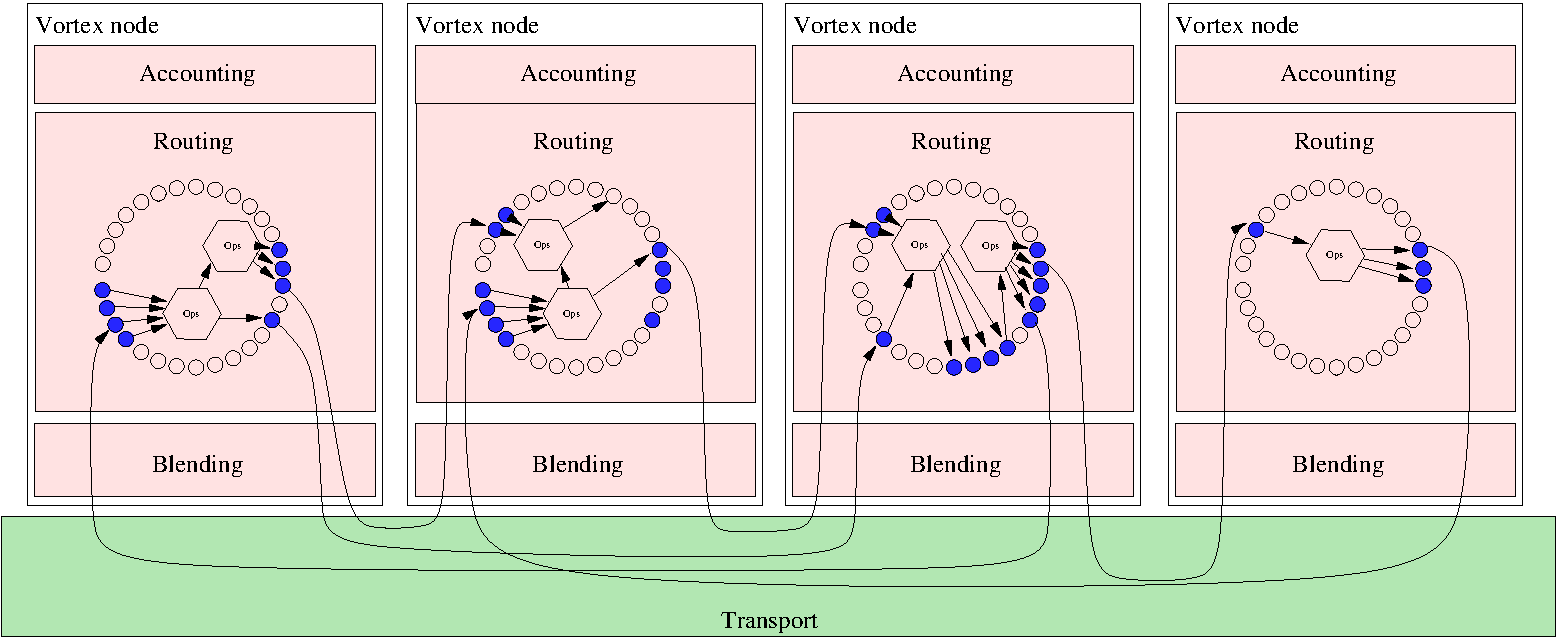
\includegraphics[width=2.5in]{../inc/roughProtocolDesign}
%\caption{Protocol stack.}
%\label{fig:layers}
%\end{figure}
The protocol is described precisely in \cite{MessageVortexRFC}. All necessary details to implement the protocol have been defined in this document. 

The protocol is divided into the three layers blending (embedding vmessages into transport), routing (processing vmessages), and accounting (prevents misuse and DoS). These three layers are connected via the fourth layer (transport). The transport layer is based on one or more store-and-forward based, common internet transport protocols. All cryptographic operations such as encryption, decryption, hashing, or random number generation within the protocol do not rely on a single algorithm. The protocol can signal what capabilities a node has and how exactly a message should be processed. This makes the protocol very robust if a used algorithm is broken. 

\subsection{Protocol Layers}
The transport layers provide the Internet infrastructure. Unlike in most other approaches such as \cite{tor-design,sherwood2005p5,freenet}, this layer is not protocol specific. We use already existing, symmetrically built store and forward protocols. Attributes such as anonymity do not rely on the security of this layer. Protocols on this layer are typically well known and frequently used. They have no prerequisite for encryption or privacy and are store-and-forward based protocols with routing capabilities. 

The blending layer embeds vmessages from the routing layer in transport protocol messages. Incoming vmessages are extracted from the transport layer and passed to the routing layer. Messages can be identified by picking up a potential vmessage and start deciphering $k_{p_N}$ using its private key $k^{-1}_{h_N}$. If decryption succeeds, a vmessage is found. Protocol features such as anonymity or redundancy do not rely on this level. This layer embeds messages within the transport layer in such a way that an adversary is no longer able to identify vmessages from regular transport layer messages. Good blending is achieved if transport layer censorship measurements such as application-level firewalls are unable to detect the difference between real-world messages and vmessages. In an ideal application, this applies to human  and algorithmic censorship. 

The routing layer is the mixer of the system. It processes messages extracted by the blending layer and is supported by the accounting layer. The routing layer processes vmessages by recombining payload with defined operations. 

The accounting layer protects a node from being overloaded or misused. Every sender must first apply for an ephemeral identity which is limited by lifetime. Nodes must apply a proof-of-work to their messages to get quotas or ephemeral identities. The ephemeral identity is assigned with message and size transfer quotas. 

\subsection{Message Processing}
We define a protocol block which has an inner block structure as shown in Fig~\ref{fig:blocks}.

\begin{figure}[htb]
	\centering
	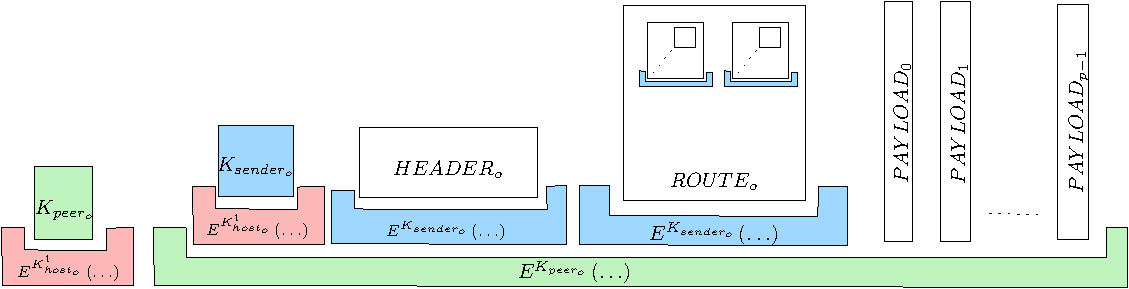
\includegraphics[width=0.8\columnwidth]{../../inc/blockLayoutSimplified}
	\caption{Protocol block outline.}
	\label{fig:blocks}
\end{figure}

These blocks are passed from node to node. Every block is protected by two symmetric keys $key_{peer_N}$ (in short $k_{p_N}$) , $key_{sender_N}$ (in short $k_{s_N}$) and the private part of an asymmetric host key $k^{-1}_{host_N}$ (in short $k^{-1}_{h_N}$). The public host key $k^{1}_{h_N}$ and both symmetric keys are known to the builder of the routing block structure. 

The header is protected by the symmetric key $k_{s_N}$ and is found in a preamble to the header protected by the receiving peer's private key $k^{-1}_{h_N}$. The key $k_{s_N}$ is known to the routing block builder and the receiving node only. The receiving node obtains all vital information protected by this key. $k_{p_N}$ is known to two immediate peers and the builder of the routing block. The sending peer obtains $k_{p_N}$ from the routing block, whereas the receiving peer acquires it in the $headerBlock$. The header block contains vital static information for the message disclosed to only one peer of the network. It is protected by key $k_{s_N}$. The operations within the routing block are designed in such a way that they allow a variance of message size without telling anyone which message part is used later. 

All interactions are non-interactive. Interactive operations such as DC-nets do add more complexity to the system. Behavioral analysis can be used to identify interactive operations. This is one of the main reasons, why DC-nets are rarely used in this context. Theoretically, it is possible to reflect them as a single operation by calculating the answer and then broadcasting the answer. In practice, this fails due to the non-existence of efficient, reliable multicast networks. There are attempts to apply DC-nets to real protocols \cite{Corrigan-Gibbs:2010:DAA:1866307.1866346}. The protocol features multiple types of operations to enable mixing. Especially noteworthy is the $addRedundancy$ operation. It supports the generation of decoy traffic in such a way that the generating node cannot tell decoy apart from real traffic. It is based on a modified Reed-Solomon redundancy function. The general inner workings are described in Fig~\ref{fig:addRedundancy}.

\begin{figure}[htb]
	\centering
	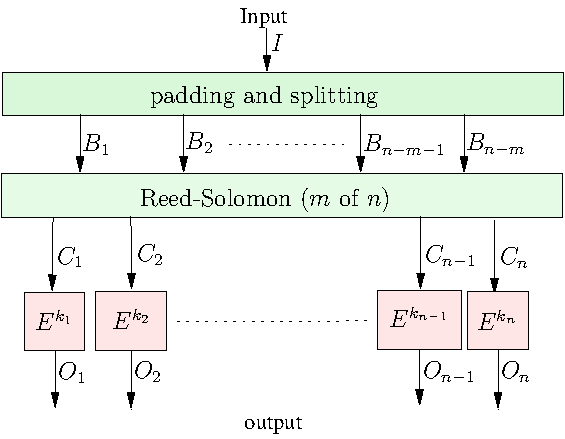
\includegraphics[width=2.5in]{../../inc/addRedundancyOp}
	\caption{AddRedundancy Operation}
	\label{fig:addRedundancy}
\end{figure}

We define a function $\addRedundancy_{n,m}( \mathbf{M},k_1\ldots k_{m} )$ where $M$ denotes the message, $n$ the number of total output blocks, $m$ the number of redundancy blocks whereas $m<n$, $k$ the encryption key and scheme to be used, and $bs_k$ the block size required to accommodate scheme and key size described by $k$. It is important to note that any set of blocks with the size of $d=n-m$ may be used to recover the full set of original data blocks. The $n$ output blocks are encrypted with the keys $k_1$-$k_n$. The message is length-prefixed with a big-endian 64 bit unsigned integer number and padded in such a way that $8+\len(M)+\len(padding) \bmod bs_k =0$. As padding stream, we take the output of $\prng_i\left(\left\lceil\frac{8+\len(M)}{b_s}\right\rceil b_s n\right )$. The first 64 bytes of the message (padded with 0 if required) are taken as initializer $i$ for the PRNG function.

Furthermore, the protocol offers support for onionized encryption, and block splitting and merging.

\subsection{Message Building}
Using previously defined operations, we may build a message path. This path is typically built by first assigning an identity set $I_k$ where  $k$ denotes the target identity. $I_k$ is a static set of $n$ ephemeral identities $I_k\langle eI_1 \ldots eI_n\rangle$ which are always used to communicate with $k$. This set may be enriched with further $m$ ephemeral identities when sending. An identity set is replaced with a different one as soon as ephemeral identities expire. Therefore, we apply a new anonymity set unrelated to the old one with each new set of ephemeral identities. A full message graph including all traffic may have any complexity. Graphs feature partially independent routes from source to the target. 

When building the message, it has to be ensured that all nodes in $I_k$ obtain enough information to rebuild the message. If an adversary is capable of identifying the full message flow and knows all the operations applied to the message except for those on the entry and exit node, and at least a subset of $k=|I_{k_{uncompromised}}|$ where $k>1$ exists then we are still at $k$-Anonymity as an absolute worst case scenario. Thus, we can prove that attacks, as described in \cite{DanSer04}, are of limited use. 

\section{Results}
Our protocol may is a toolset for creating and sending anonymized messages. The degree of anonymity and redundancy is controlled when building the routing a building node must do this with care. The protocol has been proven to be very secure against common attacks. In our thesis\cite{messageVortex} we analyze various kinds of attacks, such as illicit behaving nodes, hijacking of header and routing blocks, analysis on payload blocks, traffic replay, analysis of infrastructure, and analysis on operations. Results have shown that the protocol is very resistant against most kinds of attacks. We can  prove the effectiveness of replay protection even when assuming misbehaving nodes. Hijacking a routing block allows at worst to reduce quotas of the routing block owner. Exchanging routing or header blocks results in breaking of the message\'s path. We can easily show the effectiveness of the tagging and bugging protection. A misbehaving node has no room to tag a message without compromising the message's integrity. A tagged message will be discarded at the first non-misbehaving node. If an interruption of a path is suspected, parts of the message may be obtained by the message block builder at any time. He may do this by introducing fixed diagnostic paths into a routing block, which we refer to as implicit diagnosis, or he may send a second message picking up a block of the message at a node to be tested. We refer to this as explicit diagnostic. Explicit diagnostics may be used as a kind of ``receipt'' from any node including but not limited to the terminal receiver of a message. Any block at any time of routing may be returned directly or indirectly to the original sender. The arrival of such a packet and content tells the sender at which point a message failed. If a diagnostic packet does not arrive, the routing block builder may build a diagnostic message picking up random packets on any suspected failing node.

\section{Discussion}

\subsection{Comparison to Existing Systems}
The following section gives a short comparison to existing systems. It shows that the solution defined in this paper covers a different approach and what problems are solved. It is important to note that this is not a ranking. It just outlines the differences between the system and shows where our system is different compared to existing solutions.

Researchers criticised TOR for several things. Firstly, it is easy attackable if a transported connection is not  encrypted and authenticated. It relies on the trust in a centralized directory infrastructure. It is susceptible if more than $\approx 30\%$ of the nodes are controlled by an adversary as shown in \cite{jansen2014sniper}. Furthermore, timing analysis on entry and exit nodes are particularly easy because TOR is a low latency network\cite{torta05,esorics10-bandwidth}. Harvesting of nodes is possible (e.g., \url{https://torstatus.blutmagie.de}). Tor nodes are easily identifiable by traffic as shown in \cite{foci12-winter}. To avoid this detection TOR uses ``pluggable transports.'' between dedicated node tuples. MessageVortex tries to address these problems in multiple ways. First, there is no central infrastructure which defies the trust problem. There are no entry or exit nodes as all participating members are routers at the same time. Therefore, all problems related to entry and exit nodes do not exist. There is no dedicated transport protocol making the presence of vmessages hard to detect. MessageVortex has several downsides compared to TOR. It is not suitable for real-time communication due to its asynchronous operation. It is furthermore a closed system and only participating members may use it. 

$\mathcal{P}^5$ experienced so far very little in-depth analysis, as there is no precise protocol specification but only a rough outline available. This outline specifies the messaging and the crypto operations only. It claims to be peer to peer, which would result in NAT (Network Address Translation) circumvention technology. This technology usually relies, at least partially, on a central infrastructure (e.g., for hole punching). In contrast, MessageVortex protocol is peer to peer, but the transport layer is not. It misuses already existing infrastructure for transport. This makes it not susceptible to approaches against infrastructure unless our messages are identified and filtered. This may be corrected by applying different blending schemes for the transport layer. It furthermore removes the need for NAT hole punching and similar technologies.

$I^2P$ has not attracted as much attention as TOR so far. It is thus hard to judge its real qualities. Unlike TOR, anonymity is not fully granted. Instead, pseudonymity is used. In \cite{pets2011-i2p} an attack specific to $I^2P$ is presented. As $I^2P$s security model is chosen based on IP addresses, the authors propose to use several cloud providers in different B-Class networks. By selectively flooding peers, an adversary may extract statistical information. The paper proposes an attack based on the heuristic performance-based peer selection. The main criticism of the paper was that the peer selection might be influenced by an adversary enabling him to recover data on a statistical base. MessageVortex does only allow a routing block builder to choose routes and amount of traffic. Due to the replay protection and the trust model, we do not rely on any node. We show in \cite{messageVortex} that attacks on this level are ineffective.

Freenet is not a messaging but a distributed storage system. It has many useful features adapted by MessageVortex. Like in Freenet a MessageVortex node may deny being the owner of specific information unless the key for the respective ephemeral identity can be found on the system. As the key is only required for building routing blocks but not for message assembly and sending, this makes it a valuable feature comparable to the deniability of Freenet.

\section{Conclusion}
The MessageVortex protocol outlined in the previous sections does not solve all privacy issues which might arise. Furthermore, it is complicated to implement and involves a considerable amount of bookkeeping at runtime which is left to the sender of a message and the mixing nodes. 

On the positive side, we have a new protocol which addresses privacy in a holistic approach leaving minimal attack surface. If handled with appropriate care by the sender and receiver, the protocol allows a sender-controlled, high degree amount of anonymity. Message paths are diagnosable, may be built redundant and do not build on the trust of any third party systems including all involved mixes except the senders and receivers. Even closed group communication or broadcasting to multiple identities involving a specific subset of mixes is possible if desired by the sender.

In \cite{messageVortex} we show that the protocol is very secure. It is hard to block as messages may be redundant, hard to identify as messages are covered within message flows which may not be blocked without a massive impact on existing systems. It is hard to apply censorship in a real-world scenario as messages are tough to detect. 

MessageVortex has some flaws which must be outlined. We always considered algorithmic censorship. If human censorship is applied, we must assume that at least some of the messages are being identified as potential MessageVortex messages. If we assume a white-listing, human, censoring adversary (everything which is not identified by a human as compliant is censored) we must conclude that at least some messages will fail to be delivered.  Some of the participating transport nodes may be identified and blocked. These flaws may be compensated with redundancy in message transmission. Messages transported by MessageVortex generate vast amounts of decoy traffic. Unlike other systems which control decoy traffic on a ``per peer'' base, MessageVortex does not dynamically reduce decoy traffic as decoy traffic is not identifiable. This results in a considerable traffic overhead.


% if have a single appendix:
%\appendix[Proof of the Zonklar Equations]
% or
%\appendix  % for no appendix heading
% do not use \section anymore after \appendix, only \section*
% is possibly needed

% use appendices with more than one appendix
% then use \section to start each appendix
% you must declare a \section before using any
% \subsection or using \label (\appendices by itself
% starts a section numbered zero.)
%
% you can choose not to have a title for an appendix
% if you want by leaving the argument blank

% use section* for acknowledgement

%
% ---- Bibliography ----
%
% BibTeX users should specify bibliography style 'splncs04'.
% References will then be sorted and formatted in the correct style.
%
\bibliographystyle{splncs04}
% \bibliography{mybibliography}
\bibliography{../../inc/bib/unclassified/Anonbib/anonbib,../../messagevortex}

%
%\begin{thebibliography}{8}
%\end{thebibliography}
\end{document}
